% !TEX root = main.tex
Following the same set-up as Figure~\ref{fig:80}, Figure~\ref{fig:four-pdfs} includes the percentage of misclassifications for the considered algorithms with different preset auto-deletion threshold. Moreover, we include a new algorithm, loss-weighted scheduling, that modifies $\conbacid$ by prioritizing admitted content with largest estimated loss $\bar{\ell}$ for review. As shown in these figures, our algorithm $\conbacid$ consistently outperforms $\staticTh$, a heuristic following \cite{Avadhanula2022}, and $\bacid$ w. OfflineML (when the review ratio is larger than $0.02$). In addition, loss-weighted scheduling can further improve the efficiency of $\conbacid$.
\begin{figure}[htbp]
  \centering
  %--- 1st panel ---------------------------------------------------
  \begin{subfigure}[b]{0.24\textwidth}
    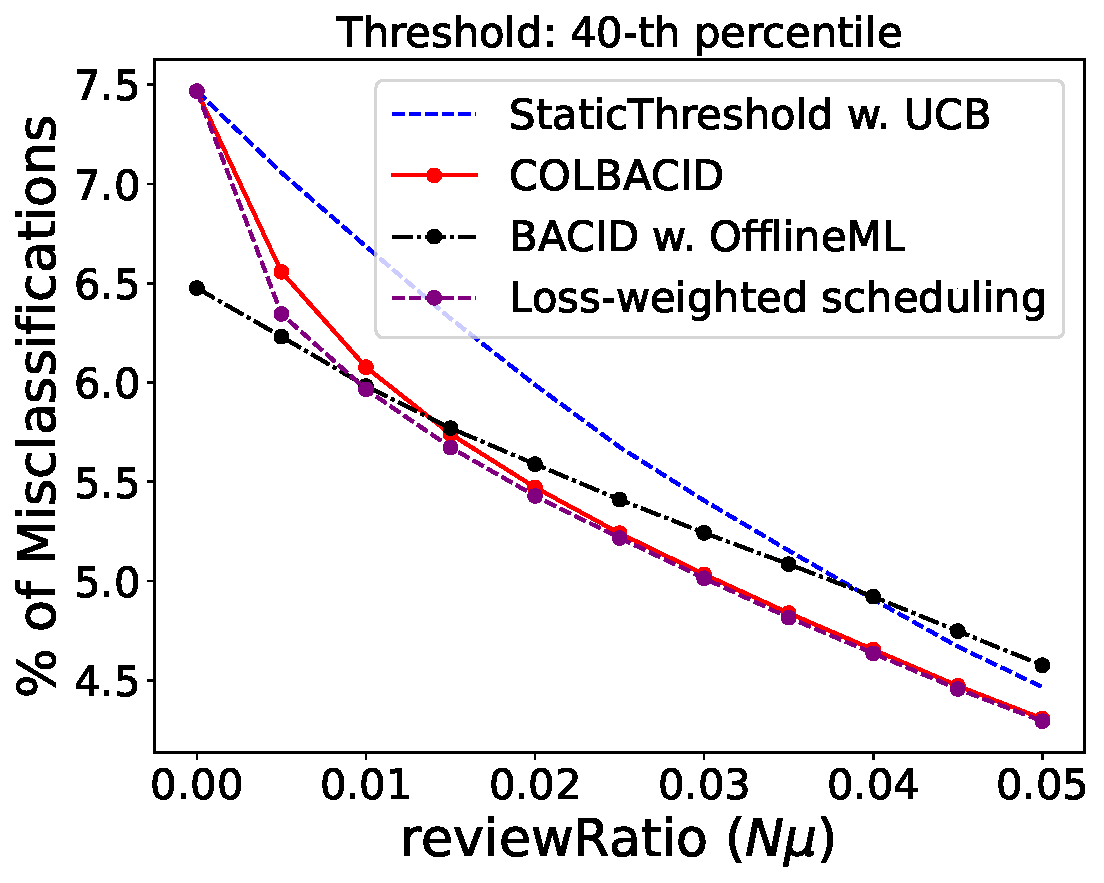
\includegraphics[width=\linewidth]{figures/40-withprio.pdf}
  \end{subfigure}\hfill
  %--- 2nd panel ---------------------------------------------------
  \begin{subfigure}[b]{0.24\textwidth}
    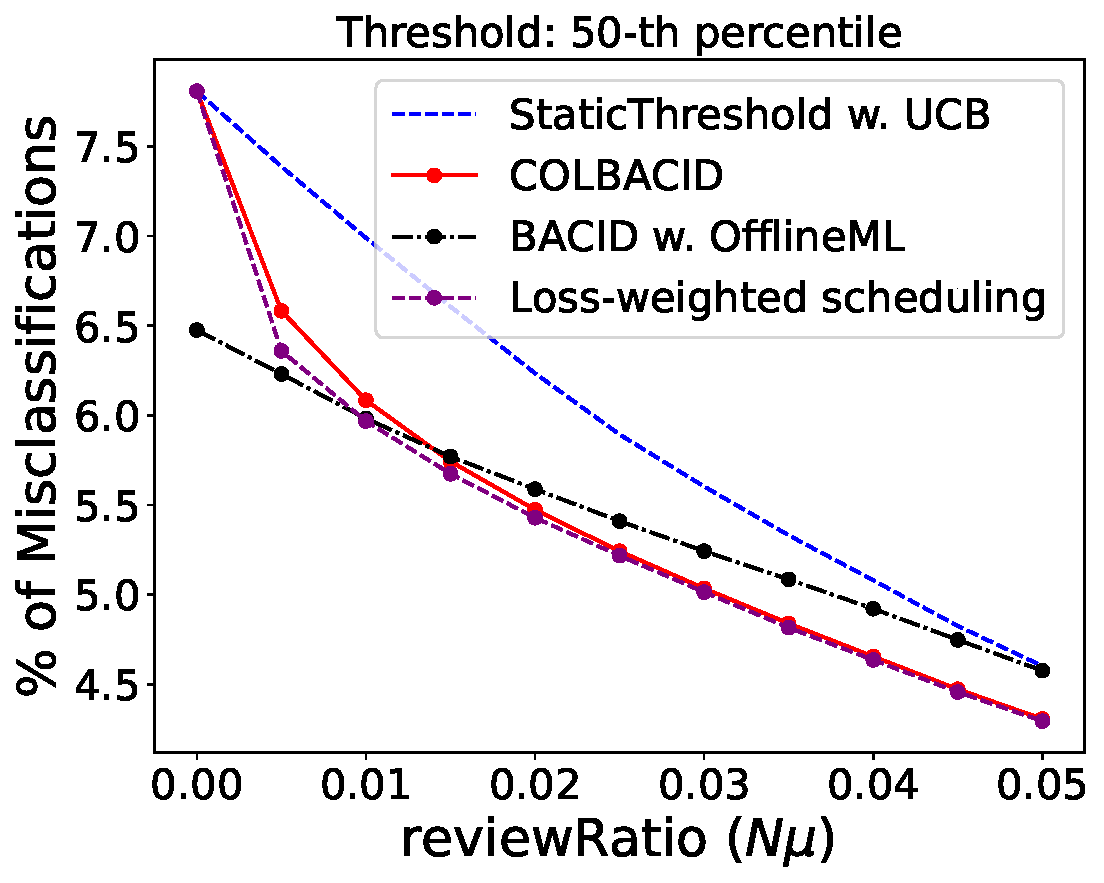
\includegraphics[width=\linewidth]{figures/50-withprio.pdf}
  \end{subfigure}\hfill
  %--- 3rd panel ---------------------------------------------------
  \begin{subfigure}[b]{0.24\textwidth}
    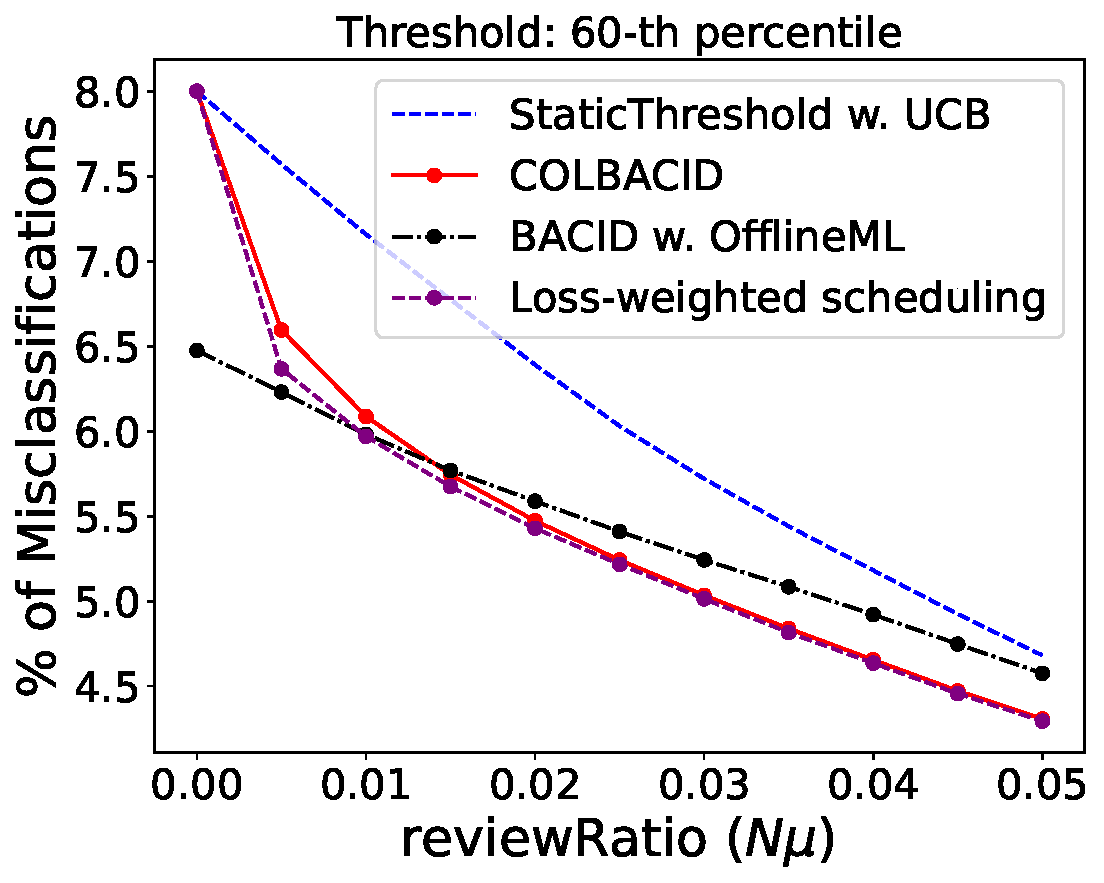
\includegraphics[width=\linewidth]{figures/60-withprio.pdf}
  \end{subfigure}\hfill
  %--- 4th panel ---------------------------------------------------
  \begin{subfigure}[b]{0.24\textwidth}
    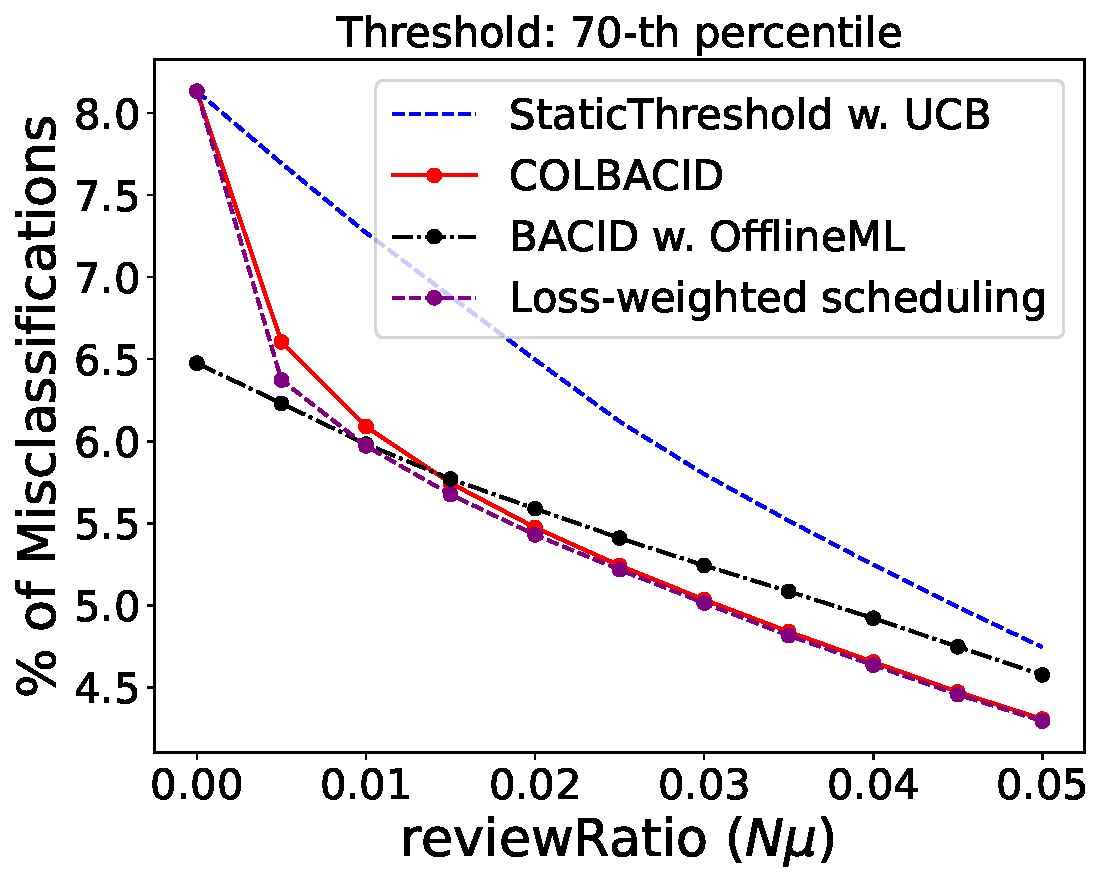
\includegraphics[width=\linewidth]{figures/70-withprio.pdf}
  \end{subfigure}

  \caption{Algorithms' percentage of misclassifications for different auto-deletion threshold}
  \label{fig:four-pdfs}
\end{figure}